%%%% ijcai19-multiauthor.tex

\typeout{speech2phone}

% These are the instructions for authors for IJCAI-19.

\documentclass{article}
\pdfpagewidth=8.5in
\pdfpageheight=11in
% The file ijcai19.sty is NOT the same than previous years'
\usepackage{ijcai19}

% Use the postscript times font!
\usepackage{times}
\usepackage{soul}
\usepackage{url}
\usepackage[hidelinks]{hyperref}
\usepackage[utf8]{inputenc}
\usepackage[small]{caption}
\usepackage{graphicx}
\usepackage{amsmath}
\usepackage{booktabs}
\usepackage{todonotes}
\urlstyle{same}

% the following package is optional:
%\usepackage{latexsym} 

% Following comment is from ijcai97-submit.tex:
% The preparation of these files was supported by Schlumberger Palo Alto
% Research, AT\&T Bell Laboratories, and Morgan Kaufmann Publishers.
% Shirley Jowell, of Morgan Kaufmann Publishers, and Peter F.
% Patel-Schneider, of AT\&T Bell Laboratories collaborated on their
% preparation.

% These instructions can be modified and used in other conferences as long
% as credit to the authors and supporting agencies is retained, this notice
% is not changed, and further modification or reuse is not restricted.
% Neither Shirley Jowell nor Peter F. Patel-Schneider can be listed as
% contacts for providing assistance without their prior permission.

% To use for other conferences, change references to files and the
% conference appropriate and use other authors, contacts, publishers, and
% organizations.
% Also change the deadline and address for returning papers and the length and
% page charge instructions.
% Put where the files are available in the appropriate places.

\title{\textit{speech2phone}: Phoneme Segmentation and Classification from Raw Audio}

\author{
Seong-Eun Cho$^1$\and
Jared Nielsen$^1$\and
Kyle Roth$^1$\\
\affiliations
$^1$Brigham Young University\\
\emails
scj1420@gmail.com,
jaredtnielsen@gmail.com,
kylrth@gmail.com
}

\begin{document}

\maketitle

\begin{abstract}
We extend the speech recognition problem by converting raw audio data into discrete phonemes, rather than directly into language. Our algorithm, \textit{speech2phone}, is a multilingual general-purpose speech preprocessor. We combine classical machine learning techniques such as dimensionality reduction with the expressive power of deep neural nets, achieving impressive results on the TIMIT dataset. Our primary contribution is combining the UMAP embedding with semi-supervised learning algorithms, achieving state-of-the-art accuracy with limited labeled data.
\end{abstract}

\section{Introduction}
Speech recognition is a fundamental discipline of computational linguistics. It has traditionally been a very difficult problem to solve even with statistical models, but has recently seen marked improvement through the use of neural networks. Similar to speech recognition, phoneme recognition is the challenge of transcribing audio inputs into a phonetic alphabet, e.g. the International Phonetic Alphabet (IPA). This has value beyond speech recognition as it can help identify certain demographics of the speaker and provides valuable insight to field linguists. In the first section of this project, we use several classical machine learning models as baselines, and demonstrate how various embedding algorithms enhance the results of those models.

The more impressive part of this project is to build a semi-supervised deep learning model. While supervised learning requires labels for all training data and unsupervised learning requires none, semi-supervised learning seeks to capitalize on both the labels of the labeled set and the generality of the (usually larger) unlabeled set. We test various statistical methods, such as principal component analysis and embedding spaces.

\section{Background}

Automatic phonetic transcription has been attempted by \cite{1}, \cite{2}, and many others, but was limited in scope and didn’t use neural networks. \cite{3} used temporal flow networks to achieve 80\% accuracy, but on a dataset of only 37 words spoken over 2.5 hours. Their approach used the output of an array of networks to then predict phonemes; each network was trained to estimate a specifically chosen phonetic feature.

% Comments:
% Is 40 an accuracy score or a hyperparameter?
% It sounds like you're just trying things for the heck of it before you try deep ML. 
% We should try an HMM
% is 61 classes enough?
% Why so many charts of hyperparameters?
% Abstract/intro uses big words
% Abstract gives a good overview
% "defend the data?"
% Explain cleaning of data before experiments
% "I don't understand what you're doing with phenomes *sic* :) Explain what a phoneme is. Explain the purpose. Better background.
% What is the phoneme frequency distribution? Does it follow Pareto, uniform, etc.?
% Make related work section crystal clear how we're new and novel.

\begin{itemize}
    \item add citations to .bib file
    \item semi-supervised learning
    \item Phoneme recognition
\end{itemize}

\section{Experiments and Results}

\subsection{Dataset}
We used TIMIT, a corpus of spoken sentences annotated with phoneme information. It contains 630 English speakers with 8 distinct dialects, each reading 10 sentences. While TIMIT is not publicly licensed, we obtained permission to use the dataset through a linguistics research group.
Since phoneme-annotated audio is a rarity, we apply semi-supervised learning (SSL) algorithms on an expanded, unannotated dataset of audio. There are 61 phonemes in the English language, making the classification more comparable to CIFAR-100 than MNIST. The baseline of most-common-value achieves only 4\% accuracy on TIMIT, the vowel `a`, so we do not expect to see high accuracy scores. Rather, the question is how well we can improve on established baselines such as a random forest or 1-D CNN on the labeled data.

\subsection{Approach}
We take three steps in this paper:
\begin{itemize}
    \item First, generating simple baselines. Random forest, KNN clustering.
	\item Second, supervised machine learning models. 1-D CNNs, fully-connected networks, RNNs.
    \item Third, semi-supervised machine learning models. We apply the Pi-Model, Label Gradient Alignment, and compare various embedding algorithms as a preprocessor. Embedding algorithms we will use are PCA, t-SNE, first half of a VAE, first half of an autoencoder, UMAP. We expect the VAE and UMAP embeddings to perform best.
\end{itemize}

\subsection{Hyperparameter Search}
Hyperparameter selection is of paramount importance. Some techniques, in order of increasing quality, are manual search, grid search, random search, and Bayesian optimization. Manual search, also called graduate student descent, involves a human sitting trying one configuration, then trying another, and so on. Grid search tries a grid of various hyperparameter configurations. Random search tries random combinations within the grid, and has been shown to perform better than grid search \cite{}. Bayesian optimization uses prior evaluations to construct a probability distribution (such as a Gaussian mixture model) over the hyperparameter space, similar to the multi-armed bandit problem. Bayesian optimization has been shown to produce superior results, so we use it via the \textit{hyperopt} package. 

\subsection{ClassicAl ML algorithms}
We applied Bayesian hyperparameter optimization to many classical machine learning algorithms, and the best results are shown in \ref{tab:classical-results}

\begin{itemize}
    \item support vector classification (SVC)
    \item random forest
    \item boosted trees
    \item feed-forward neural network
    \item quadratic discriminant analysis
    \item na\"ive Bayes
    \item logistic regression
    \item K-nearest neighbors
    \item K means
    \item Gaussian mixture
\end{itemize}
The best results achieved by each baseline model are compared in Figure \ref{tab:baseline-results}.

\begin{table}
\centering
\begin{tabular}{|c|c|}
    \hline
    Model & Accuracy \\
    \hline
    logistic regression & 0.3457 \\
    \hline
    FCNN & 0.3484 \\
    \hline
    random forest & 0.4150 \\
    \hline
    XGBoost & 0.3494 \\
    \hline
    KNN & 0.3770 \\
    \hline
    QDA & 0.2319 \\
    \hline
\end{tabular}
\caption{Accuracy scores for baseline models}
\label{tab:baseline-results}
\end{table}

\begin{figure}
    \centering
    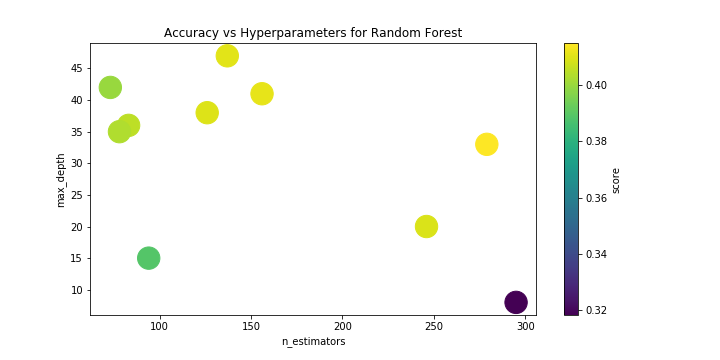
\includegraphics[width=\linewidth]{visualizations/rf.png}
    \caption{Hyperparameter search for randomforest}
    \label{fig:classical-results}
\end{figure}

\begin{figure}
    \centering
    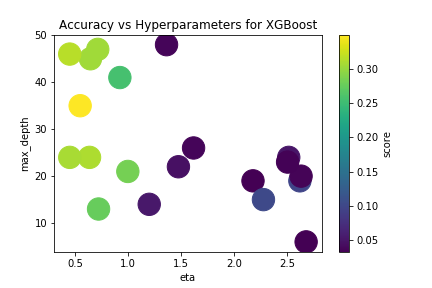
\includegraphics[width=\linewidth]{visualizations/xgb.png}
    \caption{Hyperparameter search for XGBoost}
    \label{fig:classical-results}
\end{figure}

\begin{figure}
    \centering
    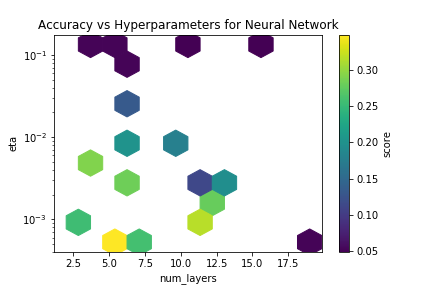
\includegraphics[width=\linewidth]{visualizations/nn.png}
    \caption{Hyperparameter search for Neural Network}
    \label{fig:classical-results}
\end{figure}

\begin{figure}
    \centering
    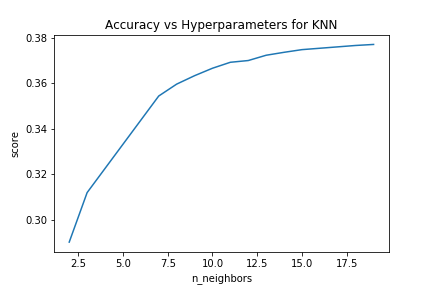
\includegraphics[width=\linewidth]{visualizations/knn.png}
    \caption{Hyperparameter search for KNN}
    \label{fig:classical-results}
\end{figure}

\section{Ethical Implications}

To our knowledge, all data has been collected in an ethical way, from speakers who either
\begin{itemize}
    \item provided informed consent for their spoken audio to be used for research purposes, or
    \item spoke in a public setting (e.g. an interview recorded and published on YouTube), where the right to control over the use of recordings is not assumed.
\end{itemize}

Since it's possible to automatically recognize the individual phonemes from audio, it's also possible to recognize the identity of speaker. Depending on the use of the model in a real-world system, speaker identification could be unethically used to identify and make decisions affecting the speaker, without his or her informed consent. We doubt that our model could be used for effective speaker identification because the purpose of the embedding is to represent the same phoneme the same way (regardless of the speaker). Nonetheless, we plan on doing experiments to see whether our model is sensitive to the identity of the speaker.

\todo{cite https://www.forbes.com/sites/realspin/2016/10/06/voice-recognition-every-single-day-every-word-you-say here?}

\section{Conclusion}


\end{document}

